\documentclass{article}

\usepackage[top=0.6in, bottom=0.75in, left=0.625in, right=0.625in]{geometry}
\usepackage{subcaption}
\usepackage[unicode]{hyperref}
\usepackage{amsmath,amsthm,amssymb}
\usepackage[utf8x]{inputenc}
\usepackage[russianb]{babel}
\usepackage{mathtools}
\usepackage{calc}
\usepackage{xcolor}
\usepackage{url}
\usepackage[nottoc,numbib]{tocbibind}
\usepackage{listings}
\usepackage{caption}
\usepackage[section]{placeins}
\usepackage{tikz}
\usepackage{pdfpages}
\usepackage{placeins} % to break floats
\usepackage{flafter}  % to break floats
\usepackage{cleveref} % nice \cref{} instead of plain \ref{}
% \usepackage{algorithm2e}
\usepackage[ruled,vlined]{algorithm2e}
\newcommand\mycommfont[1]{\ttfamily\textcolor{blue}{#1}}
\SetCommentSty{mycommfont}
\usetikzlibrary{arrows.meta}
% \captionsetup[figure]{labelformat=empty}
\usepackage[nottoc]{tocbibind}
% \usepackage{biblatex}

\usepackage{graphicx}
\graphicspath{ {./img/} }

\usepackage{tocloft}
\renewcommand\cftsecleader{\cftdotfill{\cftdotsep}}


\DeclarePairedDelimiter\ceil{\lceil}{\rceil}
\DeclarePairedDelimiter\floor{\lfloor}{\rfloor}
% \DeclareMathSymbol{*}{\mathbin}{symbols}{"01}


\SetKw{Break}{break}


\DeclareMathOperator{\di}{d\!}
\newcommand*\Eval[3]{\left.#1\right\rvert_{#2}^{#3}}

\DeclareMathOperator{\didi}{d\!}
\newcommand*\Evalat[2]{\left.#1\right\rvert_{#2}}

\DeclareMathOperator{\dididi}{d\!}
\newcommand*\littleo[1]{\overline o\left(#1\right)}

\DeclareMathOperator{\didididi}{d\!}
\newcommand*\bigo[1]{O\left(#1\right)}

\newcommand{\RN}[1]{
\textup{\uppercase\expandafter{\romannumeral#1}}
}

\newcommand{\squad}{
    \hspace{0.5em}
} 

\newcommand{\Abs}[1]{\left| #1 \right|}

\newcommand{\alignedoverset}[2]{
% #1 = over
% #2 = under
\settowidth\oversetwidth{$\overset{#1}{#2}$}
\settowidth\underwidth{$#2$}
\setlength\oversetwidth{\oversetwidth-\underwidth}
\hspace{.5\oversetwidth}
&
\settowidth\oversetwidth{$\overset{#1}{#2}$}
\settowidth\underwidth{$#2$}
\setlength\oversetwidth{\oversetwidth-\underwidth}
\hspace{-.5\oversetwidth}
\overset{#1}{#2}
}


% \newenvironment{theorem}[2][Theorem]{\begin{trivlist}
% \item[\hskip \labelsep {\bfseries #1}\hskip \labelsep {\bfseries #2.}]}{\end{trivlist}}
% \newenvironment{lemma}[2][Lemma]{\begin{trivlist}
% \item[\hskip \labelsep {\bfseries #1}\hskip \labelsep {\bfseries #2.}]}{\end{trivlist}}
% \newenvironment{claim}[2][Claim]{\begin{trivlist}
% \item[\hskip \labelsep {\bfseries #1}\hskip \labelsep {\bfseries #2.}]}{\end{trivlist}}
% \newenvironment{problem}[2][Problem]{\begin{trivlist}
% \item[\hskip \labelsep {\bfseries #1}\hskip \labelsep {\bfseries #2.}]}{\end{trivlist}}
% \newenvironment{proposition}[2][Proposition]{\begin{trivlist}
% \item[\hskip \labelsep {\bfseries #1}\hskip \labelsep {\bfseries #2.}]}{\end{trivlist}}
% \newenvironment{corollary}[2][Corollary]{\begin{trivlist}
% \item[\hskip \labelsep {\bfseries #1}\hskip \labelsep {\bfseries #2.}]}{\end{trivlist}}

% \newenvironment{solution}{\begin{proof}[Solution]}{\end{proof}}


\makeatletter
\let\@msm@th@eqref\eqref
\renewcommand{\eqref}[1]{%
  \begingroup
  \leavevmode
  \color{violet}%
  \hypersetup{linkbordercolor=[named]{violet}}%
  \@msm@th@eqref{#1}%
  \endgroup
}
\makeatother


% \newtheorem{corollary}{Предложение}[section]
\newtheorem{theorem}{Теорема}
\newtheorem{lemma}{Лемма}
\newtheorem{corollary}{Предложение}
\newtheorem{definition}{Определение}
\newtheorem{note}{Замечание}

\allowdisplaybreaks



\begin{document}

\tableofcontents

\pagebreak

\section{Введение}

\subsection{Конструкция}

Рассмотрим ориентированный метрический граф (одномерный клеточный комплекс). Каждое ребро его является гладкой регулярной кривой и имеет длину, а также разрешенное направление движения. Мы будем рассматривать ситуацию общего положения и предполагать, что все длины ребер линейно независимы над полем рациональных чисел. Также зафиксируем вершину, которую будем называть стартовой.


В нулевой момент времени из стартовой вершины вдоль всех ребер, которые из нее выходят, начинают двигаться точки с единичной скоростью. Как только какая-то из точек оказывается в вершине, на каждом инцидентном вершине ребре появляется новая точка, которая начинает двигаться в сторону конца ребра, а старая исчезает. Если в одну вершину одновременно приходит сразу несколько точек, то все эти точки пропадают, а появляются новые точки так, как это было описано для одной точки.


Пусть $N(T)$ --- количество движущихся точек в момент времени $T$. Основной нашей целью является изучение данной функции на различных графах.

Данная динамическая конструкция уже была рассмотрена для неориентированных графов (см. \cite{poly}, \cite{second}). Для числа движущихся точек было получено полиномиальное приближение, то есть приведено описание многочлена степени $E - 1$, где $E$ – число ребер графа, который аппроксимирует $N(T)$ с точностью до некоторой степени логарифма. В самое последнее время для некоторых ориентированных графов (one-way Sperner graph в \cite{2021}) был получен старший член асимптотики.

Мы же будем рассматривать произвольные ориентированные гамильтоновы графы.



\subsection{Структура текста и рассматриваемые графы}


\begin{definition} $ $
    \begin{enumerate}
        \item Пусть $N(T)$ --- сколько точек находится на графе в момент времени $T$.
        \item Пусть $N_{x}(T)$ --- сколько есть моментов времени $\leq T$, что в вершину номер $x$ заходили точки.
    \end{enumerate}
\end{definition}

Основная задача --- найти $N(T)$ для графов, которые будут описаны далее.

Будем рассматривать ориентированные гамильтоновы графы c $n = |V|$.
Считаем, что процесс начинается из вершины номер $1$ и длины всех ребер линейно независимы над $\mathbb{Q}$. 

\begin{figure}[!htb]
\begin{center}
\tikzstyle{circ node}=[circle,draw=black]
\tikzstyle{arrow style}=[->,-{Latex[width=2mm]}]
\begin{tikzpicture}[minimum size=1cm, scale=3]
    \node[circ node,draw=green] (1) at (0 * 90:1cm) {$1$};
    \node[circ node] (2) at (1 * 90:1cm) {$2$};
    \node[circ node] (3) at (2 * 90:1cm) {$3$};
    \node[circ node] (4) at (3 * 90:1cm) {$4$};

    \draw[arrow style] (1) edge node {} (2);
    \draw[arrow style] (2) edge node {} (3);
    \draw[arrow style] (3) edge node {} (4);
    \draw[arrow style] (4) edge node {} (1);

    \draw[arrow style] (4) edge[bend right=30] node {} (1);
    \draw[arrow style] (2) edge[bend left=30] node {} (1);
    \draw[arrow style] (4) edge[bend left=30] node {} (3);
    \draw[arrow style] (1) edge node {} (3);
\end{tikzpicture}
\caption{Пример гамильтонова графа с выделенной стартовой вершиной}
\label{fig:graph}  
\end{center}
\end{figure}

Раздел $3.1$ показывает, что достаточно представить $N_{1}(T)$ в виде
\begin{gather*}
N_{1}(T) = aT^{\beta} + bT^{\beta - 1} + O(T^{\beta - 2}), \squad \beta = |E| - |V| + 1,    
\end{gather*} 
чтобы получить $N(T)$.

Разделы $2.1, 2.2, 2.3$ посвящены нахождению нужного представления для произвольного графа, описанного в разделе $1.2$. Раздел $2.4$ показывает как получить коэффициент более явным образом.

Раздел $3.2$ соединяет полученные из $3.1$ и $2.1, 2.2, 2.3$ знания и дает итоговую формулу для $N(T)$.


% Далее такие графы будем называть гамильтоновыми графами.



\section{Классификация путей в стартовую вершину}

\subsection{Алгоритм}

Поскольку граф гамильтонов, то для каждой вершины $i$ есть ребро в следующую вершину: для $i \in \{1, \ldots, n - 1\}$ это $i + 1$, а для $n$ это $1$. 
Будем называть такие ребра внутренними (если таких ребер несколько для вершины $i$, то берем любое). Цикл из внутренних ребер --- внутренний цикл. Остальные ребра будут внешними. Цикл с внешним ребром --- внешний цикл.

Для каждой вершины рассмотрим выходящие из нее ребра. Зафиксируем на них порядок так, чтобы внутреннее ребро было последним.

Рассмотрим пример.

\begin{figure}[!htb]
\begin{center}
\tikzstyle{circ node}=[circle,draw=black]
\tikzstyle{arrow style}=[->,-{Latex[width=2mm]}]
\begin{tikzpicture}[minimum size=1cm, scale=3]
    \node[circ node,draw=green] (1) at (0 * 90:1cm) {$1$};
    \node[circ node] (2) at (1 * 90:1cm) {$2$};
    \node[circ node] (3) at (2 * 90:1cm) {$3$};
    \node[circ node] (4) at (3 * 90:1cm) {$4$};

    \draw[arrow style] (1) edge[draw=red] node {} (2);
    \draw[arrow style] (2) edge[draw=red] node {} (3);
    \draw[arrow style] (3) edge[draw=red] node {} (4);
    \draw[arrow style] (4) edge[draw=red] node {} (1);

    \draw[arrow style] (4) edge[bend right=30] node {} (1);
    \draw[arrow style] (2) edge[bend left=30] node {} (1);
    \draw[arrow style] (4) edge[bend left=30] node {} (3);
    \draw[arrow style] (1) edge node {} (3);
    \begin{scope}[yshift=-1.5cm]
        \node[text width=6cm] at (0, 0) {{\color{red} Красным} выделены внутренние ребра, черным выделены внешние ребра};
    \end{scope}
    \begin{scope}[xshift=3cm]
        \node[circ node,draw=green] (1) at (0 * 90:1cm) {$1$};
        \node[circ node] (2) at (1 * 90:1cm) {$2$};
        \node[circ node] (3) at (2 * 90:1cm) {$3$};
        \node[circ node] (4) at (3 * 90:1cm) {$4$};

        \draw[arrow style] (1) edge node[left] {{\color{red} 2}} (2);
        \draw[arrow style] (2) edge node[right] {{\color{blue} 2}} (3);
        \draw[arrow style] (3) edge node[right] {{\color{magenta} 1}} (4);
        \draw[arrow style] (4) edge node[left] {{\color{orange} 3}} (1);

        \draw[arrow style] (4) edge[bend right=30] node[right] {{\color{orange} 1}} (1);
        \draw[arrow style] (2) edge[bend left=30] node[right] {{\color{blue}1}} (1);
        \draw[arrow style] (4) edge[bend left=30] node[left] {{\color{orange} 2}} (3);
        \draw[arrow style] (1) edge node[auto] {{\color{red} 1}} (3);
        \begin{scope}[yshift=-1.5cm]
            \node[text width=6cm] at (0, 0) {Возможный порядок на ребрах, последнее ребро из любой вершины --- внутреннее ребро};
        \end{scope}
    \end{scope}
\end{tikzpicture}
\caption{Внешние и внутренние ребра, порядок на ребрах}    
\end{center}
\end{figure}

\FloatBarrier

Красным выделены внутренние ребра, черным внешние, все внутренние ребра образуют гамильтонов цикл.

\begin{definition} $ $
    \begin{enumerate}
        \item Пусть $\mathcal{H}$ --- множество всех таких графов $H$, в которых те же ребра и вершины, что и в $G$, но на каждом ребре написано неотрицательное целое число так, что для любой вершины сумма чисел на входящих ребрах равна сумме чисел на выходящих.
        \item $c = a + b$ для $a \in \mathcal{H}, \squad b \in \mathcal{H}$ будет такой граф $c \in \mathcal{H}$, что у него на каждом ребре написана сумма чисел соответствующих ребер $a$ и $b$.
        \item $c = \alpha b$ для $b \in \mathcal{H}, \squad \alpha \in \mathbb{N}$ будет такой граф $c \in \mathcal{H}$, что у него на каждом ребре написано произведение числа для соответствующего ребра в $b$ и $\alpha$.
    \end{enumerate} 
\end{definition}

Смысл числа на ребре --- сколько раз по нему прошли. Сумма входящих равна сумме выходящих означает, что в каждую вершину зашли и вышли одинаковое число раз.
Множество $\mathcal{H}$ дальше понадобится для того, чтобы запускать алгоритм на графах из этого множества.


Опишем алгоритм, который разбивает $H \in \mathcal{H}$ на циклы определенного вида.
Пусть $H' = H$. В $H'$ будут меняться числа на ребрах и отметки по ходу алгоритма.
\begin{center}
    \textit{Алгоритм разбиения пути на циклы}
\end{center}

\begin{center}
\fbox{\begin{minipage}{40em}
\texttt{Шаг 1. Начиная из вершины $1$, каждый раз выбираем первое неотмеченное ребро. Когда приходим в вершину, в которой уже были, полагаем $c$ -- образованный цикл.} \\

\texttt{Шаг 2. Пока в графе $H'$ все ребра вдоль цикла $c$ больше $0$, вычитаем $1$ вдоль них и берем цикл $c$ в ответ.} \\

\texttt{Шаг 3. Если цикл $c$ -- внутренний и нулевой, то останавливаемся.} \\
\texttt{       Иначе отмечаем первое нулевое внутреннее ребро в цикле $c$. Возвращаемся к шагу 1.} \\

\end{minipage}}
\end{center}

\begin{figure}[!htb]
\begin{center}
\begin{tikzpicture}[minimum size=0.7cm, scale=0.8, baseline=(current bounding box.center)]
    \node[shape=circle,draw=black] (0) at (0, 0) {$2$};
    \node[shape=circle,draw=green] (3) at (0, 3) {$1$};
    \node[shape=circle,draw=black] (2) at (0, -3) {$3$};
    
    \draw [, -{Latex[width=2mm]}] (3) edge [bend left] node[right]  {$3$} (0);
    \path [blue,-{Latex[width=2mm]}] (3) edge [bend right] node[right] {$2$} (0);
    \path [, -{Latex[width=2mm]}] (0) edge [bend left] node[right] {$1$} (2);
    \path [blue,-{Latex[width=2mm]}] (0) edge [bend right] node[right] {$4$} (2);
    \path [blue, -{Latex[width=2mm]}] (2) edge [bend left=50] node[right] {$5$} (3);   
\end{tikzpicture} \squad $\longrightarrow$ \squad
\begin{tikzpicture}[minimum size=0.7cm, scale=0.8, baseline=(current bounding box.center)]
    \node[shape=circle,draw=black] (0) at (0, 0) {$2$};
    \node[shape=circle,draw=green] (3) at (0, 3) {$1$};
    \node[shape=circle,draw=black] (2) at (0, -3) {$3$};
    
    \draw [blue, -{Latex[width=2mm]}] (3) edge [bend left] node[right]  {$3$} (0); 
    \path [-{Latex[width=2mm]}] (3) edge [bend right] node[right] {$0$} (0);
    \path [-{Latex[width=2mm]}] (0) edge [bend left] node[right] {$1$} (2);
    \path [blue, -{Latex[width=2mm]}] (0) edge [bend right] node[right] {$2$} (2);
    \path [blue, -{Latex[width=2mm]}] (2) edge [bend left=50] node[right] {$3$} (3);   
\end{tikzpicture}
\squad $\longrightarrow$ \squad
\begin{tikzpicture}[minimum size=0.7cm, scale=0.8, baseline=(current bounding box.center)]
    \node[shape=circle,draw=black] (0) at (0, 0) {$2$};
    \node[shape=circle,draw=green] (3) at (0, 3) {$1$};
    \node[shape=circle,draw=black] (2) at (0, -3) {$3$};
    
    \draw [blue, -{Latex[width=2mm]}] (3) edge [bend left] node[right]  {$1$} (0);
    \path [, -{Latex[width=2mm]}] (3) edge [bend right] node[right] {$0$} (0);
    \path [blue,-{Latex[width=2mm]}] (0) edge [bend left] node[right] {$1$} (2);
    \path [, -{Latex[width=2mm]}] (0) edge [bend right] node[right] {$0$} (2);
    \path [blue, -{Latex[width=2mm]}] (2) edge [bend left=50] node[right] {$1$} (3);   
\end{tikzpicture}
\squad $\longrightarrow$ \squad
\begin{tikzpicture}[minimum size=0.7cm, scale=0.8, baseline=(current bounding box.center)]
    \node[shape=circle,draw=black] (0) at (0, 0) {$2$};
    \node[shape=circle,draw=green] (3) at (0, 3) {$1$};
    \node[shape=circle,draw=black] (2) at (0, -3) {$3$};
    
    \draw [-{Latex[width=2mm]}] (3) edge [bend left] node[right]  {$0$} (0);
    \path [-{Latex[width=2mm]}] (3) edge [bend right] node[right] {$0$} (0);
    \path [-{Latex[width=2mm]}] (0) edge [bend left] node[right] {$0$} (2);
    \path [-{Latex[width=2mm]}] (0) edge [bend right] node[right] {$0$} (2);
    \path [-{Latex[width=2mm]}] (2) edge [bend left=50] node[right] {$0$} (3);   
\end{tikzpicture}
\end{center}
\caption{Пример работы алгоритма}
\label{example_algo}
\end{figure}


\begin{lemma} (Корректность алгоритма)
\label{lemma:algo}

Пусть мы запускаем алгоритм на $H \in \mathcal{H}$, $c$ --- любой цикл, который получается в ходе алгоритма, 

$H' \in \mathcal{H}$ --- то, что <<осталось>> от $H$ после нескольких шагов алгоритма.
\begin{enumerate}
\item Если в ходе алгоритма в $c$ есть нулевое ребро, то либо в $c$ есть внешнее нулевое ребро, либо $c$ --- внутренний цикл. 
\item Алгоритм разобьет $H$ на циклы так, что все ребра в $H'$ в конце алгоритма будут нулевыми.
\end{enumerate}
\end{lemma}
\begin{proof}
Для доказательства утверждений нам понадобится простое, но полезное наблюдение о том, что в ходе алгоритма сохраняется инвариант, что в любой вершине сумма входящих ребер равна сумме выходящих.


\begin{enumerate}
    \item Пусть $e = (v, u)$ --- нулевое ребро в $c$. Если оно внешнее, тогда все доказано. Предположим, что оно внутреннее. Поскольку внутреннее ребро --- последнее среди выходящих из вершины, то ребро $e$ --- последнее из $v$, к тому же вес $e$ --- $0$, поэтому все ребра из $v$ имеют нулевой вес (ребра до $e$ имеют нулевой вес, поскольку они отмечены, а отмечаются только ребра нулевого веса). В силу инварианта, все ребра в $v$ также нулевого веса и соответственно ребро $e' = (w, v)$ цикла $c$ тоже нулевого веса. Если оно внешнее, то доказано, иначе оно внутреннее и можно продолжить аналогичные рассуждения. В рассуждениях мы идем сначала от вершины $v$ к $v - 1$, потом $v - 2, \ldots, 1$, $n, \ldots, v + 1$ и показываем, что либо очередное ребро внутреннее и продолжаем, либо ребро внешнее и останавливаемся. Если ни одно ребро не оказалось внутренним, то получается, что $c$ --- внутренний цикл с нулевыми ребрами. 
    \item Пункт (1) показывает корректность $\texttt{шага 3}$, и что алгоритм завершится (в какой-то момент будут пройдены внешние циклы, потом будет пройден внутренний цикл).
    Поскольку алгоритм в какой-то момент доходит до внутреннего цикла, то все внешние ребра будут равны $0$, внутренние будут равны $0$ после этапа алгоритма, который выделяет внутренний цикл.
\end{enumerate}
\end{proof}

\subsection{Генерируемые и достижимые наборы циклов}


Во всех дальнейших обозначениях считаем, что $c_{i}$ --- простой цикл в графе $G$.

\begin{definition}
    Набор $(c_{1}, c_{2}, \ldots, c_{k})$ назывется полным набором генерируемых циклов, если $c_{1}$ получен с использованием $\texttt{шага 1}$ без отмеченных ребер, а для остальных выполнено $c_{1} \xrightarrow{v_{1}} c_{2} \xrightarrow{v_{2}}c_{3}\xrightarrow{v_{3}} \ldots, \xrightarrow{v_{k - 1}}c_{k}$. То есть $c_{j}$ был получен из $c_{j - 1}$ отмечанием первого неотмеченного внешнего ребра в $v_{j - 1}$ и запуском $\texttt{шага 1}$. Этот процесс продолжается пока есть внешние неотмеченные ребра.
\end{definition}

\begin{definition}
    Пусть $\beta = |E| - |V| + 1$.
\end{definition}

Далее нам понадобится следующее наблюдение: в полном наборе достижимых циклов всегда ровно $\beta$ циклов. Это верно, потому что каждому циклу кроме последнего можно сопоставить биективно внешнее ребро, которое было отмечено после прохождения этого цикла. Всего внешних ребер $|E| - |V|$, но осталось учесть последний внутренний цикл, таким образом, всего $|E| - |V| + 1 = \beta$ циклов в полном наборе. 



% \begin{corollary}
%     Аналогично можно переформулировать определение набора генерируемых циклов$c_{1}$ получен с использованием $\texttt{шага 1}$ без отмеченных ребер, а для остальных выполнено $c_{1} \xrightarrow{v_{1}}\ldots\xrightarrow{v_{i_{1}}} c_{2} \xrightarrow{v_{i_{1} + 1}}\ldots\xrightarrow{v_{i_{2}}}c_{3} \ldots c_{k - 1}\xrightarrow{v_{i_{k - 2} + 1}}\ldots\xrightarrow{v_{\beta}}c_{k}, \squad i_{j} < i_{j + 1}$. То есть $c_{j}$ был получени из $c_{j - 1}$ отмечанием соответствующих ребер в $v_{i_{j - 2} + 1} \ldots v_{i_{j - 1}}$ и запуском $\texttt{шага 1}$.
% \end{corollary}

\begin{definition} $ $
    \label{gen}
    \begin{enumerate}
        \item Набор $(c_{1}, c_{2}, \ldots, c_{k})$ назывется набором генерируемых циклов, если $(c_{1}, \ldots, c_{k})$ --- подпоследовательность какого-то полного набора генерируемых циклов.
        \item Набор $((c_{1}, a_{1}), (c_{2}, a_{2}), \ldots, (c_{k}, a_{k}))$ назывется набором взвешенных генерируемых циклов, если $(c_{1}, c_{2}, \ldots, c_{k})$ --- набор генерируемых циклов, $a_{i} \in \mathbb{N}$.
    \end{enumerate}
\end{definition}

\begin{definition} $ $
    \begin{enumerate}
        \item Временем пути $P = (e_{1}, \ldots, e_{k})$ будем считать $t(P) = \sum_{i = 1}^{k}{t(e_{i})}$.
        \item Временем набора взвешенных генерируемых циклов $c = ((c_{1}, a_{1}), (c_{2}, a_{2}), \ldots, (c_{k}, a_{k}))$ называется $t(c) = \sum_{i = 1}^{k}{a_{i}t(c_{i})}$.
    \end{enumerate} 
\end{definition}


\begin{definition} $ $
    \label{def:omega}
    \begin{enumerate}
        \item Введем функцию $\sigma$. По лемме \eqref{lemma:algo} алгоритм задает отображение, которое сопоставляет $H \in \mathcal{H}$ взвешенный набор генерируемых циклов $c$. Будем называть это отображние $\sigma$.
        \item Введем функцию $\omega$. Пусть $T = \sum_{i = 1}^{|E|}{a_{i}t(e_{i})}, \squad a_{i} \in \mathbb{N} \cup \{0\}$. Построим граф $H$, в котором на ребре $e_{i}$ написано $a_{i}$. Определим $\omega(T) = H$.
        \item Введем функцию $\mu = \sigma \circ \omega$.
    \end{enumerate}
\end{definition}

Функция $\sigma$ <<запускает>> на графе 
$H \in \mathcal{H}$ алгоритм и выдает результат.

Функция $\omega$ дает по времени граф, у которого есть информация сколько раз по каждому ребру прошли. 
В определении $\omega$ граф существует в силу выбора $T$, на которых определена функция $\omega$ и $\omega(T)$ задан единственным образом в силу линейной независимости над $\mathbb{Q}$ ребер.
Следует обратить внимание на то, что функция $\omega$ определена не для любых времен, а только для времен особого вида.

Функция $\mu$ сохраняет время, то есть $t(\mu(T)) = t(\sigma(\omega(T))) = T$, если $\omega(T) \in \mathcal{H}$ и $T = \sum_{i = 1}^{|E|}{a_{i}t(e_{i})}, \squad a_{i} \in \mathbb{N} \cup \{0\}$. Это немедленно следует из леммы \eqref{lemma:algo}.



\begin{definition}
    Пусть $\mathcal{T}$ --- множество всех времен захода в стартовую вершину.
\end{definition}

% Вообще, чтобы посчитать $N_{1}(T)$ нас интересуют времена захода путей из стартовой вершины в нее же, а не $t(H)$ для произвольных $H \in \mathcal{H}$, но следующее предложение показывает, что если мы посчитаем все   


\begin{corollary}
    \label{corollary:generated}
    Из леммы \eqref{lemma:algo} следует, что любое время $T \in \mathcal{T}$ можно представить как 
    $\sum_{i = 1}^{k}{a_{i}t(c_{i})} = t(c)$, где $c = ((c_{1}, a_{1}), \ldots, (c_{k}, a_{k}))$ --- набор взвешенных генерируемых циклов. Действительно, давайте предъявим такое $c$. По выбору $T$, $T$ можно представить как $\sum_{i = 1}^{|E|}{a_{i}t(e_{i})}, \squad a_{i} \in \mathbb{N} \cup \{0\}$, то есть можно взять $H = \omega(T)$. Поскольку $T \in \mathcal{T}$, то $H \in \mathcal{H}$. Возьмем $c = \mu(T)$, тогда $t(c) = t(\mu(T)) = T$, и мы получили набор такой набор взвешенных генерируемых циклов $c$, что $t(c) = T$.
\end{corollary}


Предложение \eqref{corollary:generated} показывает, что мы можем сопоставить времени $T \in \mathcal{T}$ взвешенный набор генерируемых циклов $c$ со временем $T$ c помощью $\mu$, но обратное неверно. То есть если взять произвольный набор взвешенных генерируемых циклов $c$, то не обязательно существует $\mu^{-1}(c)$. 

Теперь мы хотим это исправить и сделать так, чтобы между $\mathcal{T}$ и каким-то множеством наборов взвешенных генерируемых циклов была биекция задаваемая функцией $\mu$. Заметим, что инъекция уже есть. Действительно, разные $T_{1} \neq T_{2}$ будут давать $\mu(T_{1}) \neq \mu(T_{2})$, поскольку 
$t(\mu(T_{1})) = T_{1}$, $t(\mu(T_{2})) = T_{2}$ и $T_{1} \neq T_{2}$ по предположению.  Для биекции осталось получить сюръекцию, но ее просто сделать: необходимо ограничить множество всех взвешенных генерируемых циклов до $\mu(\mathcal{T})$.

Получается, что есть какое-то <<хорошее>> множество наборов взвешенных генерируемых циклов. 

По определению $N_{1}(T) = \#\{t \in \mathcal{T}: t \leq T\}$. 
Также справедливо
$\#\{t \in \mathcal{T}: t \leq T\}$ = 

\noindent
$\#\{c \text{ --- <<хороший>> набор взвешенных генерируемых циклов}: t(c) \leq T\}$, в силу того, что есть биекция между $\mathcal{T}$ и множеством <<хороших>> наборов взвешенных генерируемых циклов $\sigma$, которая сохраняет
время.

Таким образом, вместо понятия <<хороший>> набор взвешенных генерируемых циклов, целесообразно ввести новое определение.

\begin{definition} $ $
    \label{def:reachable_weighted_simple}
    
    Набор $c = ((c_{1}, a_{1}), (c_{2}, a_{2}), \ldots, (c_{k}, a_{k}))$ назывется набором взвешенных достижимых циклов, если
    \begin{enumerate}
         \item Набор $c$ является набором взвешенных генерируемых циклов.
         \item $c \in \mu(\mathcal{T})$  
    \end{enumerate}
\end{definition}

В доказательствах будет удобнее использовать эквивалентное определение.


\begin{definition} (Эквивалентное определение взвешенного набора достижимых циклов)
    \label{def:reachable_weighted}

    Набор $c = ((c_{1}, a_{1}), (c_{2}, a_{2}), \ldots, (c_{k}, a_{k}))$ является набором взвешенных достижимых циклов тогда и только тогда, когда
    \begin{enumerate}
         \item Набор $c$ является набором взвешенных генерируемых циклов.
         \item $\mu(t(c)) = c$.
         \item Если оставить все положительные ребра в $\omega(t(c))$, то получится сильно связный граф, который проходит через вершину $1$. 
    \end{enumerate}
\end{definition}

Смысл условия $2$ определения \eqref{def:reachable_weighted} в том, что набор $c$ будет получаться как результат алгоритма на $\omega(t(c))$. В этом смысле он <<достижим>>.

Условие $3$ определения \eqref{def:reachable_weighted} эквивалентно тому, что набор $c$ задает путь из $1$ в себя.


\begin{lemma}
    \label{lemma:induction}
    Если $c = ((c_{1}, a_{1}), (c_{2}, a_{2}), \ldots, (c_{k}, a_{k}))$ --- набор взвешенных достижимых циклов, то 

    \noindent
    $c' = ((c_{1}, b_{1}), (c_{2}, b_{2}), \ldots, (c_{k}, b_{k})), \squad b_{i} \in \mathbb{N}$ тоже набор взвешенных достижимых циклов.
\end{lemma}
\begin{proof} $ $
    
    Первое условие выполнено по определению набора взвешенных генерируемых циклов, третье выполнено, потому что множество ненулевых ребер в $\omega(t(c))$ и $\omega(t(c'))$ одинаково.

    Осталось показать, что выполнено второе условие. Пусть $d = \mu(t(c'))$, $d = ((d_{1}, x_{1}), \ldots, (d_{k}, x_{k}))$. Нужно показать $c' = d$.
    Поскольку $c$, $d$ --- наборы взвешенных генерируемых циклов, то допустимо следующее представление:
    \begin{align*}
         \sigma = &\xrightarrow{V_{0}} (c_{1}, a_{1}) \xrightarrow{V_{1}} (c_{2}, a_{2}) \ldots (c_{k - 1}, a_{k - 1}) \xrightarrow{V_{k - 1}} (c_{k}, a_{k}), \squad V_{i} = (V_{i}^{1} \ldots V_{i}^{s_{i}}) \lor \varnothing \\
         \omega = &\xrightarrow{U_{0}} (d_{1}, x_{1}) \xrightarrow{V_{1}} (d_{2}, x_{2}) \ldots (d_{k - 1}, x_{k - 1}) \xrightarrow{U_{k - 1}} (d_{w}, x_{w}), \squad U_{i} = (U_{i}^{1} \ldots U_{i}^{p_{i}}) \lor \varnothing \\
    \end{align*}

    Пусть алгоритм прошел до $(d_{i}, x_{i}), \squad i \in \{1, \ldots, w\}$ в $d$, взял цикл $d_{i}$ $x_{i}$ раз и остановился, тогда
    \begin{enumerate}
        \item $i \leq k$, $\forall j \leq i \squad d_{j} = c_{j}$, $x_{j} = b_{j}$ \\
        \item Состояние алгоритма (для всех вершин первое неотмеченное ребро) равно состоянию алгоритма, если бы он прошел до $(c_{i}, a_{i})$ в $c$, взял цикл $c_{i}$ $a_{i}$ раз и остановился.
    \end{enumerate}
    Докажем это по индукции.

    База $i = 0$:

    Первое утверждение очевидно выполнено. Второе выполнено, поскольку изначально одинаковое состояние.

    \medskip

    Переход. Пусть выполнено для $i$, докажем для $i + 1$:

    Пусть $G_{c} = \omega(t(c)), \squad G_{d} = \omega(t(d)) = \sum_{j = 1}^{w}{x_{j}d_{j}}$. По определению $d$, $G_{d} = \omega(t(c'))$. Также пусть $G_{d}^{i}$ --- граф, который получился после прохождения алгоритма до $(d_{i}, x_{i})$ включительно, аналогично определяется $G_{c}^{i}$.
    Заметим следующее:
    \begin{align*}
        G_{d}^{i} &= \sum_{j = i + 1}^{w}{x_{j}d_{j}} \\
                  &= \sum_{j = 1}^{w}{x_{j}d_{j}} - \sum_{j = 1}^{i}{x_{j}d_{j}} \\ 
                  &= \left[\text{По предположению индукции}\right] \sum_{j = 1}^{w}{x_{j}d_{j}} - \sum_{j = 1}^{i}{b_{j}c_{j}} \\
                  &= G_{d} - \sum_{j = 1}^{i}{b_{j}c_{j}} \\
                  &= \omega(t(c')) - \sum_{j = 1}^{i}{b_{j}c_{j}} \\
                  &= \sum_{j = 1}^{k}{b_{j}c_{j}} - \sum_{j = 1}^{i}{b_{j}c_{j}} \\
                  &= \sum_{j = i + 1}^{k}{b_{j}c_{j}} \\
    \end{align*}

    Поскольку в $G_{d}^{i} = \sum_{j = i + 1}^{k}{b_{j}c_{j}}$ есть ненулевые ребра, то $k \geq i + 1$.
    Заметим, что поскольку $G_{c}^{i} = \sum_{j = i + 1}^{k}{a_{j}c_{j}}$, то в $G_{c}^{i}$ и $G_{d}^{i}$ совпадает множество ненулевых ребер. Рассмотрим $V_{i} = (V_{i}^{1} \ldots V_{i}^{s_{i}})$ и $U_{i} = (U_{i}^{1} \ldots U_{i}^{p_{i}})$. Поскольку состояния одинаковые после $(c_{i}, a_{i})$ в $c$ и $(d_{i}, x_{i})$ в $d$ и множество нулевых ребер одинаковое, то циклы в данный момент будут одинаковыми и отметка пойдет на одни и те же ребра, то есть $V_{i}^{1} = U_{i}^{1}$. Заметим, что опять состояние одинаковое, мы не поменяли числа на ребрах, поэтому так же множество нулевых ребер совпадает, то есть $V_{i}^{2} = U_{i}^{2}$. Не может быть так, что $s_{i} \neq p_{i}$, потому что тогда бы в каком-то цикле было нулевое ребро, а в том же цикле но в другом наборе оно было бы ненулевым, то есть $V_{i} = U_{i}$. То есть мы дошли до $(c_{i + 1}, a_{i + 1})$ и $(d_{i + 1}, x_{i + 1})$. Поскольку $V_{i} = U_{i}$, то состояние одинаковое, то есть $c_{i + 1} = d_{i + 1}$.

    $G_{d}^{i} = b_{i + 1}c_{i + 1} + \sum_{j = i + 2}^{k}{b_{j}c_{j}}$. Если $k = i + 1$, то $G_{d}^{i} = b_{i + 1}c_{i + 1}$ и $x_{i + 1} = b_{i + 1}$, иначе посмотрим на ребро, которое было отмечено $V_{i + 1}^{1}$. Оно входит в цикл $c_{i + 1}$ и используется ровно $b_{i + 1}$ раз. Все остальные ребра цикла используются $\geq b_{i + 1}$ раз. То есть цикл $c_{i + 1}$ будет вычитаться ровно $b_{i + 1}$ раз, $x_{i + 1} = b_{i + 1}$.

    \medskip

    Получаем, что $k \geq w, \squad \forall j \leq w$ $c_{j} = d_{j}, \squad x_{j} = b_{j}$. То есть $d$ --- префикс $c'$, если $k > w$, 
    то $\omega(t(c')) \neq \omega(t(d))$, таким образом $k = w$ и $c' = d$. 
\end{proof}


\begin{definition}
    \label{def:reachable}
    Набор $(c_{1}, c_{2}, \ldots, c_{k})$ называется набором достижимых циклов, если $((c_{1}, 1), (c_{2}, 1), \ldots, (c_{k}, 1))$ является набором взвешенных достижимых циклов.  
\end{definition}

Смысл определения \eqref{def:reachable} в том, что если $(c_{1}, c_{2}, \ldots, c_{k})$ --- набор достижимых циклов, то любой взвешенный набор с этимим циклами является взвешенным достижимым, и наоборот, если $(c_{1}, c_{2}, \ldots, c_{k})$ является генерируемым, но не достижимым, то любой взвешенный набор не будет взвешенным достижимым. Это верно в силу леммы \eqref{lemma:induction}.


\begin{definition}
    $D_{k}$ --- множество всех наборов достижимых циклов длины $k$.
\end{definition}

\subsection{Формула для \texorpdfstring{$N_{1}(T)$}{}}

\begin{theorem}
\label{theorem:N_1}
    \begin{gather*}
        N_{1}(T) = \sum_{i = 1}^{\beta}{\sum_{d \in D_{i}}{\#\left\{\sum_{j = 1}^{i}{n_{j}t(d_{j}) \leq T, \squad n_{j} > 0}\right\}}}
    \end{gather*}
\end{theorem}

\begin{proof} $ $

    Вообще говоря, это уже обсуждалось, но давайте убедимся в этом еще раз.

    \medskip

    Покажем, что $N_{1}(T) \leq \sum_{i = 1}^{\beta}{\sum_{d \in D_{i}}{\#\left\{\sum_{j = 1}^{i}{n_{j}t(d_{j}) \leq T, \squad n_{j} > 0}\right\}}}$.

    Пусть $t' \leq T$ --- время захода в $1$, также по лемме \eqref{lemma:algo} $c = \mu(t')$ --- набор взвешенных генерируемых циклов. Покажем, что $c$ также набор взвешенных достижимых циклов. Поскольку $c$ задает путь в $1$, то достаточно проверить $\mu(t(c)) = c$, но 
    $c = \mu(t') \Rightarrow t(c) = t(\mu(t')) \Rightarrow t(c) = t' \Rightarrow c = \mu(t(c))$. Но суммирование $\sum_{i = 1}^{\beta}{\sum_{d \in D_{i}}{\#\left\{\sum_{j = 1}^{i}{n_{j}t(d_{j}) \leq T, \squad n_{j} > 0}\right\}}}$ учитывает все наборы взвешенных достижимых циклов, что время набора $\leq T$, но $c$ --- набор взвешенных достижимых циклов и $t(c) = t' \leq T$, то есть он учтется.  

    \medskip

    Теперь покажем, что $\sum_{i = 1}^{\beta}{\sum_{d \in D_{i}}{\#\left\{\sum_{j = 1}^{i}{n_{j}t(d_{j}) \leq T, \squad n_{j} > 0}\right\}}} \leq N_{1}(T)$. Рассмотрим два набора, которые участвуют в сумме $((c_{1}, n_{1}) \ldots (c_{k}, n_{k}))$ и $((d_{1}, n_{1}') \ldots (d_{p}, n_{p}'))$,
    $c \neq d$ . То есть $c$, $d$ --- наборы взвешенных достижимых циклов с $t(c) \leq T, \squad t(d) \leq T$.
    Оба они они задают время захода в $1$. Известно, что $c = \mu(t(c)), \squad d = \mu(t(d))$. Если $t(c) = t(d)$, то $c = d$, но $c \neq d$.

    \medskip

    Таким образом, получили искомое.
\end{proof}

\subsection{\texorpdfstring{Наборы взвешенных генерируемых циклов длины $\beta$}{}}

\begin{definition}
    Определим
    \begin{gather*}
        cnt_{[l;r]}^{c}(e) = \sum_{i = l}^{r}{a_{i} \cdot I\{e \in c_{i}\}},
    \end{gather*} 
    где $I\{X\}$ --- индикатор истинности $X$, $e \in E, \squad c = ((c_{1}, a_{1}), \ldots, (c_{p}, a_{p}))$ --- набор взвешенных достижимых циклов.
\end{definition}


\begin{lemma} $ $
    \label{lemma:eq}
        Если $c = ((c_{1}, a_{1}), \ldots, (c_{p}, a_{p}))$, $d = ((d_{1}, b_{1}), \ldots, (d_{k}, b_{k}))$ --- два набора взвешенных генерируемых циклов таковы, что $\exists i: \forall j, \squad 1 \leq j < i \squad c_{j} = d_{j} \land a_{j} = b_{j}, \squad c_{i} = d_{i} \land a_{i} \neq b_{i}$, то $t(c) \neq t(d)$.
\end{lemma}
\begin{proof} $ $
    Пусть противное, $t(c) = t(d)$. 
    Поскольку все ребра линейно независимы над $\mathbb{Q}$, то для любого $e \in E$ должно быть выполнено $cnt_{[1;p]}^{c}(e) = cnt_{[1;k]}^{d}(e)$. Посмотрим на последовательность отметок.

    Возьмем $i$ из условия. Очевидно, что $i < p \land i < k$ (аналогично случаю $v_{1} = u_{1}$. Если $i = p \land i = k$, то очевидно, иначе пусть, например, $i = p$, тогда в наборе $d$ где-то произойдет отметка, и в том ребре будет разным общее $cnt$). Посмотрим на то, как получился цикл $c_{i + 1}$ из $c_{i}$ и $d_{i + 1}$
    из $d_{i}$. Пусть для $c_{i + 1}$ произошли отметки на $v_{1}, \ldots, v_{s}$, а для $d_{i + 1}$ на $u_{1}, \ldots, u_{t}$. 

    Пусть $v_{1} = u_{1}$, обозначим за $e_{v}$ ребро, которое отметили. Получаем
    \begin{gather*}
        cnt_{[1;p]}^{c}(e_{v}) = cnt_{[1;i - 1]}^{c}(e_{v}) + a_{i} \\
        cnt_{[1;k]}^{d}(e_{v}) = cnt_{[1;i - 1]}^{d}(e_{v}) + b_{i},
    \end{gather*}
    но $cnt_{[1;i - 1]}^{c}(e_{v}) = cnt_{[1;i - 1]}^{d}(e_{v})$, а $a_{i} \neq b_{i}$ $\Rightarrow$ $cnt_{[1;p]}^{c}(e_{v}) \neq cnt_{[1;k]}^{d}(e_{v})$. Противоречие.

    Пусть теперь $v_{1} \neq u_{1}$. Ребро, которое отметили в $c$ обозначим за $e_{v}$, а в $d$ за $e_{u}$. Получаем неравенства

    \begin{equation*}
        \begin{aligned}[c]
        cnt_{[1;p]}^{c}(e_{v}) &= cnt_{[1;i - 1]}^{c}(e_{v}) + a_{i} \\
        cnt_{[1;k]}^{d}(e_{v}) &\geq cnt_{[1;i - 1]}^{d}(e_{v}) + b_{i} \\
        &\Downarrow \\
        b_{i} &\leq a_{i} \\
        \end{aligned}
        \qquad
        \begin{aligned}[c]
        cnt_{[1;k]}^{d}(e_{u}) &= cnt_{[1;i - 1]}^{d}(e_{u}) + b_{i} \\
        cnt_{[1;p]}^{c}(e_{u}) &\geq cnt_{[1;i - 1]}^{c}(e_{u}) + a_{i} \\
        &\Downarrow \\
        a_{i} &\leq b_{i} \\
        \end{aligned} 
    \end{equation*}
    Получаем $a_{i} = b_{i}$, противоречие.
\end{proof}

\begin{definition}
    Будем называть два набора взвешенных генерируемых циклов $c = ((c_{1}, a_{1}), \ldots, (c_{m}, a_{m}))$ и $d = ((d_{1}, b_{1}), \ldots, (d_{k}, b_{k}))$ одинаковыми и обозначать как $c = d$, если $m = k$ и $\forall i \leq m$ $c_{i} = d_{i}$ и $a_{i} = b_{i}$.
    В противном случае будем считать их разными и обозначать как $c \neq d$.
\end{definition}

\begin{lemma} $ $
        \label{lemma:beta}
        Если $c = ((c_{1}, a_{1}), \ldots, (c_{\beta}, a_{\beta}))$ и $d = ((d_{1}, b_{1}), \ldots, (d_{k}, b_{k})), \squad k \leq \beta$ --- два разных набора взвешенных генерируемых циклов, то $t(c) \neq t(d)$.
\end{lemma}
\begin{proof} $ $

    Для удобства сравнения записей, будем считать, что если до первого цикла нет отметок, то есть <<пустая отметка>>.
    Поскольку $d$ --- набор взвешенных достижимых циклов, то $d' = (d_{1}, \ldots, d_{k})$ --- набор генерируемых циклов, а они являются подпоследовательностью какого-то полного набора генерируемых циклов, то $d'$ можно записать как $\xrightarrow{U_{0}} d_{1} \xrightarrow{U_{1}}d_{2}\xrightarrow{U_{2}}d_{3}\ldots d_{k - 1}\xrightarrow{U_{k - 1}}d_{k}, \squad U_{i} = (U_{i}^{1},\ldots, U_{i}^{s_{i}}) \lor \varnothing$, а взвешенный набор можно записать как $\sigma = \xrightarrow{U_{0}} (d_{1}, b_{1}) \xrightarrow{U_{1}}(d_{2}, b_{2})\xrightarrow{U_{2}}(d_{3}, b_{3})\ldots (d_{k - 1}, b_{k - 1})\xrightarrow{U_{k - 1}}(d_{k}, b_{k})$.

    В свою очередь для $c$ справедливо следующее представление: 
    \begin{gather*}
        \omega = (c_{1}, a_{1}) \xrightarrow{V_{1}}(c_{2}, a_{2}) \xrightarrow{V_{2}}(c_{3}, a_{3}) \ldots (c_{\beta - 1}, a_{\beta - 1}) \xrightarrow{V_{\beta - 1}} (c_{\beta}, a_{\beta}), \squad V_{i} = (v_{i}), \squad i \in \{1, \ldots, \beta - 1\}
    \end{gather*}

    \RN{1} $U_{0} \neq \varnothing$.

    Пусть $U_{0} = (u, \ldots)$ и $e_{u}$ --- ребро, которое было отмечено после первого прохождения $u$, тогда $cnt_{[1; k]}^{d}(e_{u}) = 0$, $cnt_{[1; \beta]}^{c}(e_{u}) > 0$. Получаем $t(c) \neq t(d)$.

    \medskip

    \RN{2} $U_{0} = \varnothing$. 

    Поскольку $U_{0} = \varnothing$, то $\sigma = (d_{1}, b_{1}) \xrightarrow{U_{1}}(d_{2}, b_{2})\xrightarrow{U_{2}}(d_{3}, b_{3})\ldots (d_{k - 1}, b_{k - 1})\xrightarrow{U_{k - 1}}(d_{k}, b_{k})$. 

    Заметим, что $\sigma$ и $\omega$ состоят из двух типов объектов: $(\cdot, \cdot)$ и $\xrightarrow{\cdot}$. Будем идти слева направо и сравнивать для $(\cdot, \cdot)$ $a_{i}$ и $b_{i}$, а для $\xrightarrow{\cdot}$ будем сравнивать наборы $V_{i}$ и $U_{i}$ как мультимножества. Если таким образом $\omega$ --- собственный префикс $\sigma$, то очевидно $t(c) \neq t(d)$. 

    Иначе существует $i: a_{i} \neq b_{i} \lor V_{i} \neq U_{i}$. 

    В первом случае, когда $U_{i} = V_{i}$ и $a_{i} \neq b_{i}$ можно заметить, что $\forall j < i$ $c_{j} = d_{j} \land a_{j} = b_{j}$, $c_{i} = d_{i} \land a_{i} \neq b_{i}$. По лемме \eqref{lemma:eq}, пункт $1$ получаем, что $t(c) \neq t(d)$.

    Во втором случае $V_{i} \neq U_{i}$. Это значит, что есть внешнее ребро $e_{u}$, которое было отмечено в $d$, но пока не было отмечено в $c$, но поскольку $c$ --- полный набор взвешенных циклов, то в какой-то момент в будущем мы переключимся c этого ребра дальше, но поскольку это произойдет после $\xrightarrow{V_{i}}$, то $cnt_{[i + 1;\beta]}^{c}(e_{u}) > 0$, но $cnt_{[i + 1; k]}^{d}(e_{u}) = 0$.

    \begin{gather*}
        cnt_{[1; \beta]}^{c}(e_{u}) = cnt_{[1; i]}^{c}({e_{u}}) + \underbrace{cnt_{[i + 1; \beta]}^{c}(e_{u})}_{> 0} \\
        cnt_{[1; k]}^{d}(e_{u}) = cnt_{[1; i]}^{d}(e_{u}) + \underbrace{cnt_{[i + 1; k]}^{d}(e_{u})}_{= 0} \\
        \Downarrow \\
        cnt_{[1; \beta]}^{c}(e_{u}) \neq cnt_{[1; k]}^{d}(e_{u}) \\
        \Downarrow \\
        t(c) \neq t(d)
    \end{gather*}
\end{proof}

\begin{lemma}
    \label{lemma:beta_reachable}
    Пусть $c = (c_{1}, \ldots, c_{\beta})$ --- набор генерируемых циклов длины $\beta$,
    тогда $c$ также набор достижимых циклов длины $\beta$.
\end{lemma}
\begin{proof}
    По определению \eqref{def:reachable} достаточно проверить, что $c_{1} = ((c_{1}, 1), \ldots, (c_{\beta}, 1))$ --- набор взвешенных достижимых циклов. Для него, в свою очередь, надо проверить, что выполнены условия в определении \eqref{def:reachable_weighted}. 
    Третье условие выполнено, так как $c_{\beta}$ --- внутренний цикл, который проходит по всем вершинам. 
    Проверим второе условие. Рассмотрим $d = \mu(t(c_{1}))$, имеем $t(c_{1}) = t(d)$. Но по лемме \eqref{lemma:beta} получаем $c_{1} = d$.
\end{proof}


\pagebreak

\section{Подсчет коэффициента}

\subsection{Общие графы}

\textbf{Следующая лемма справедлива для любого ориентированного сильно связного графа $G$ с линейно независимыми над $\mathbb{Q}$ ребрами.}

Для отрезка длины $\tau$ на расстоянии $r$ от начала ребра $e$ количество точек в момент времени $T$ на нем --- $N_{\tau, e, r}(T)$.

\begin{lemma} $ $

\label{pg}
Пусть $N_{1}(T) = a_{1}T^{\beta} + b_{1}T^{\beta - 1} + O(T^{\beta - 2})$, тогда:
\begin{enumerate} 
    % \item $N_{1}(T) = a_{1}T^{\beta} + b_{1}T^{\beta - 1} + O(T^{\beta - 2})$, где $a_{1} = \sum_{d \in D_{\beta}}\frac{1}{\beta!\prod_{i = 1}^{\beta}{d_{i}}}$
    % \item $N_{i}(T) = a_{i}T^{\beta} + b_{i}T^{\beta - 1} + O(T^{\beta - 2}) \squad \forall i \in \{1, \ldots, n\}$, где $a_{i} = a_{1}$
    \item $N_{\tau, e, r}(T) = \tau \cdot a_{1} \cdot \beta \cdot T^{\beta - 1} + O(T^{\beta - 2}) \squad \forall e = (1, v) \in E$, $\tau > 0$
    \item $N_{\tau, e, r}(T) = \tau \cdot a_{1} \cdot \beta \cdot T^{\beta - 1} + O(T^{\beta - 2}) \squad \forall e \in E$, $\tau > 0$
    \item $N(T) = \left(\sum_{e \in E}{t(e)}\right) \cdot a_{1} \cdot \beta \cdot T^{\beta - 1} + O(T^{\beta - 2})$
\end{enumerate}
\end{lemma} 
\begin{proof} $ $

\begin{enumerate}
    % \item По \eqref{imp} достаточно просуммировать по всем возможным линейным комбинациям циклов достижимых наборов, но по известной асимптотической формуле, достаточно взять только все наборы длины $\beta$ и $\beta - 1$. Получаем искомое.
    % \item Есть путь от $1$ до $i$ длины $p_{1}$ и обратно длины $p_{2}$.

    % Получаем
    % \begin{gather*}
    %     N_{1}(T - p_{1}) \leq N_{i}(T) \leq N_{i}(T + p_{2}) \\
    %     a_{1}T^{\beta} + b'T^{\beta - 1} \leq N_{i}(T) \leq a_{1}T^{\beta} + b''T^{\beta - 1} \\
    %     \Downarrow \\
    %     N_{i}(T) = a_{1}T^{\beta} + O(T^{\beta - 1}) \\
    % \end{gather*}
    % \textit{Доказательства $N_{i}(T) = a_{1}T^{\beta} + b_{i}T^{\beta - 1} + O(T^{\beta - 2})$ пока нет, но, надеюсь, что скоро будет. Есть один вариант, но там много писать и он до конца не проработан.}
    \item
    Пусть $r$ --- расстояние до вершины $1$ от начала отрезка и $T' = T - r$. 
    % {\color{red} небольшой фикс нужен, нужно сделать замену переменной $T$, поскольку отрезок не обязательно в начале.}
    \begin{gather*}
        N_{\tau, e, r}(T) = N_{1}(T') - N_{1}(T' - \tau) + O(1) = a_{1}T'^{\beta} + b_{1}T'^{\beta - 1} - (a_{1}(T' - \tau)^{\beta} + b_{1}(T' - \tau)^{\beta - 1}) + O(T'^{\beta - 2}) = \\
        = \tau a_{1} \beta T'^{\beta - 1} + O(T'^{\beta - 2}) =\tau a_{1} \beta T^{\beta - 1} + O(T^{\beta - 2}) \\
    \end{gather*}
    \item
        Докажем сначала для ребер длины $\tau < t(e), \forall e \in E$.
        Отложим отрезок на ребре $e$ длины $\varepsilon$ и отрезок длины $\varepsilon$ на ребре $e_{1}$,
        которое выходит из $1$ и от которого можно дойти до $e$. Пусть от конца отрезка на ребре $e$ до конца отрезка на ребре $e_{1}$ путь длины $p_{1}$, а от конца отрезка на ребре $e_{1}$ до конца отрезка на ребре $e$ путь длины $p_{2}$.
        \begin{gather*}
            N_{\varepsilon, e_{1}, r_{1}}(T - p_{2}) \leq N_{\varepsilon, e, r_{2}}(T) \leq N_{\varepsilon, e_{1}, r_{1}}(T + p_{1}) \\
            \varepsilon a_{1} \beta T^{\beta - 1} + O(T^{\beta - 2}) \leq N_{\varepsilon, e, r_{2}}(T) \leq \varepsilon a_{1} \beta T^{\beta - 1} + O(T^{\beta - 2}) \\
            \Downarrow \\
            N_{\varepsilon, e, r_{2}}(T) = \varepsilon a_{1} \beta T^{\beta - 1} + O(T^{\beta - 2})
        \end{gather*}
        Рассмотрим остальные значения $\tau$.
        Замостим отрезок длины $\tau$ отрезками длины $\leq \min\{t(e), e \in E\}$, то есть $ \{l_{i}\}_{i = 1}^{k}, \squad \sum_{i = 1}^{k}{l_{i}} = \tau, \squad l_{i}\leq \varepsilon$.
        Получаем:
        \begin{gather*}
            N_{\tau, e, r}(T) = \sum_{i = 1}^{k}{N_{l_{i}, e, r_{i}}}(T) = \sum_{i = 1}^{k}{(l_{i} a_{1} \beta T^{\beta - 1} + O(T^{\beta - 2}))} = \left(\sum_{i = 1}^{k}{l_{i}}\right) a_{1} \beta T^{\beta - 1} + O(T^{\beta - 2}) = \tau a_{1} \beta T^{\beta - 1} + O(T^{\beta - 2})
        \end{gather*}

        \item
        $N(T)$ --- количество точек на графе в момент времени $T$, это количество можно получить как сумму количеств точек на каждом ребре в момент времени $T$. Имеем:
        \begin{gather*}
            N(T) = \sum_{e \in E}{N_{t(e), e, 0}(T)} = \left(\sum_{e \in E}{t(e)}\right) a_{1}  \beta  T^{\beta - 1} + O(T^{\beta - 2}) \\
        \end{gather*}
\end{enumerate}
\end{proof}

\begin{lemma} (равномерность распределения)

    $\frac{N_{\tau, e}(T)}{N(T)} \xrightarrow{T \to +\infty} \frac{\tau}{\sum_{e \in E}{t(e)}}$
\end{lemma}
\begin{proof} $ $

    Воспользуемся пунктами $2$ и $3$ \eqref{pg}.
    \begin{align*}
        \lim_{T \to +\infty}{\frac{N_{\tau, e}(T)}{N(T)}} = \lim_{T \to +\infty}{\frac{\tau a_{1} \beta + O\left(\frac{1}{T}\right)}{\left(\sum_{e \in E}{t(e)}\right) a_{1} \beta + O(\frac{1}{T})}} = \frac{\tau}{\sum_{e \in E}{t(e)}} \\
    \end{align*}
\end{proof}

\subsection{Гамильтоновы графы}

\textbf{Вернемся к графам из раздела $1$}
\begin{lemma}
    \label{lemma:linear_independent}
    Если $c = (c_{1}, \ldots, c_{k})$ --- набор генерируемых циклов, то $\{t(c_{1}), \ldots, t(c_{k})\}$ линейно независимы над $\mathbb{Q}$
\end{lemma}
\begin{proof} $ $

    Пусть противное и $\exists (\alpha_{1}, \ldots, \alpha_{k}) \neq (0, \ldots, 0)$, что $\sum_{i = 1}^{k}{\alpha_{i}t(c_{i})} = 0$. Можно считать, что $\alpha_{i} \in \mathbb{Z}$. Известно, что $c$ --- подпоследовательность полного достижимого набора $d$ (набора длины $\beta$). Положим $\gamma = \max_{i = 1}^{k}{|\alpha_{i}| + 1}$, получаем 
    \begin{align*}
        \sum_{i = 1}^{k}{\alpha_{i}t(c_{i})} &= 0 \\
        \sum_{i = 1}^{\beta}{\alpha_{i}'t(d_{i})} &= \sum_{i = 1}^{\beta}{\gamma t(d_{i})}, \squad \alpha_{i}' > 0 \\
    \end{align*}
    $(\alpha_{1}, \ldots, \alpha_{k}) \neq (0, \ldots, 0) \Rightarrow (\alpha_{1}', \ldots, \alpha_{\beta}') \neq (\gamma, \ldots, \gamma)$

    Противоречие лемме \eqref{lemma:beta}. 
\end{proof}

\begin{lemma} $ $
    \label{lemma:main}
    \begin{enumerate}
        \item $N_{1}(T) = a_{1}T^{\beta} + b_{1}T^{\beta - 1} + O(T^{\beta - 2})$, где $a_{1} = \sum_{d \in D_{\beta}}\frac{1}{\beta!\prod_{i = 1}^{\beta}{t(d_{i})}}$
        \item $N(T) = \left(\sum_{d \in D_{\beta}}\frac{\sum_{e \in E}{t(e)}}{(\beta - 1)!\prod_{i = 1}^{\beta}{t(d_{i})}}\right) \cdot T^{\beta - 1} + O(T^{\beta - 2})$
    \end{enumerate}
\end{lemma}
\begin{proof} $ $
    \begin{enumerate}
        \item По \eqref{theorem:N_1} имеем: 
        \begin{align*}
            N_{1}(T) &= \sum_{i = 1}^{\beta}{\sum_{d \in D_{i}}{\#\left\{\sum_{j = 1}^{i}{n_{j}t(d_{j}) \leq T, \squad n_{j} > 0}\right\}}} \\
                     &= {\sum_{d \in D_{\beta}}{\#\left\{\sum_{j = 1}^{\beta}{n_{j}t(d_{j}) \leq T, \squad n_{j} > 0}\right\}}} + \sum_{i = 1}^{\beta - 1}{\sum_{d \in D_{i}}{\#\left\{\sum_{j = 1}^{i}{n_{j}t(d_{j}) \leq T, \squad n_{j} > 0}\right\}}} \\
                     &= \left[\text{по известной асимптотической формуле и лемме \eqref{lemma:linear_independent}}\right] \\
                     &= \sum_{d \in D_{\beta}}{\frac{1}{\beta!\prod_{j = 1}^{\beta}{t(d_{j})}}} T^{\beta} + b'T^{\beta - 1} + O(T^{\beta - 2}) + b''T^{\beta - 1} + O(T^{\beta - 2}) \\
                     &= a_{1}T^{\beta} + b_{1}T^{\beta - 1} + O(T^{\beta - 2}) \\
        \end{align*}
        \item Применяем лемму \eqref{pg} и получаем, что
        \begin{align*}
            N(T) &= \left(\sum_{e \in E}{t(e)}\right) a_{1}  \beta  T^{\beta - 1} + O(T^{\beta - 2}) = \left(\sum_{e \in E}{t(e)}\right) \left(\sum_{d \in D_{\beta}}\frac{1}{\beta!\prod_{i = 1}^{\beta}{t(d_{i})}}\right)  \beta  T^{\beta - 1} + O(T^{\beta - 2}) \\ 
            &= \left(\sum_{d \in D_{\beta}}\frac{\sum_{e \in E}{t(e)}}{(\beta - 1)!\prod_{i = 1}^{\beta}{t(d_{i})}}\right) \cdot T^{\beta - 1} + O(T^{\beta - 2})
        \end{align*}
    \end{enumerate}

    По лемме \eqref{lemma:beta_reachable} можно понимать $D_{\beta}$ как множество всех генерируемых циклов длины $\beta$.
\end{proof}

\pagebreak

\section{Дополнительно}


\subsection{Случай, когда ровно один полный достижимый набор}

Пусть мы рассматриваем только гамильтоновы графы. В общем случае в $D_{\beta}$ может быть много наборов достижимых циклов.
Давайте рассмотрим частный случай гамильтоновых графов, когда есть ровно один полный достижимый набор.

Рассмотрим ориентированный цикл. Разобьем все вершины на два множества. Первое множество будет содержать вершины, номера которых идут подряд, но не будет содержать стартовую вершину. Второе множество будет содержать все остальные вершины (стартовую вершину в частности). 

Все ребра, которые находятся вне ориентированного цикла могут идти лишь из второго множества вершин в первое.

\begin{figure}[!htb]
\begin{center}
\tikzstyle{circ node}=[circle,draw=blue]
\tikzstyle{arrow style}=[->,-{Latex[width=2mm]}]
\begin{tikzpicture}[minimum size=1cm, scale=3]
    \node[circ node][draw=red] (1) at (0 * 36:1cm) {$1$};
    \node[circ node][draw=red] (2) at (1 * 36:1cm) {$2$};
    \node[circ node] (3) at (2 * 36:1cm) {$3$};
    \node[circ node] (4) at (3 * 36:1cm) {$4$};
    \node[circ node] (5) at (4 * 36:1cm) {$5$};
    \node[circ node] (6) at (5 * 36:1cm) {$6$};
    \node[circ node] (7) at (6 * 36:1cm) {$7$};
    \node[circ node] (8) at (7 * 36:1cm) {$8$};
    \node[circ node][draw=red] (9) at (8 * 36:1cm) {$9$};
    \node[circ node][draw=red] (10) at (9 * 36:1cm) {$10$};

    \draw[arrow style] (1) -- (2);
    \draw[arrow style] (2) -- (3);
    \draw[arrow style] (3) -- (4);
    \draw[arrow style] (4) -- (5);
    \draw[arrow style] (5) -- (6);
    \draw[arrow style] (6) -- (7);
    \draw[arrow style] (7) -- (8);
    \draw[arrow style] (8) -- (9);
    \draw[arrow style] (9) -- (10);
    \draw[arrow style] (10) -- (1);

    \draw[arrow style] (2) -- (8);
    \draw[arrow style] (1) -- (7);
    \draw[arrow style] (9) -- (3);
    \draw[arrow style] (9) -- (5);
\end{tikzpicture}
\caption{Пример графа, у которого ровно один полный достижимый набор}    
\end{center}
\end{figure}
{\color{blue} Синие} вершины из первого множества, {\color{red} красные} из второго.

Имеем ровно один набор полный достижимый набор, потому что в каждом простом цикле в графе не более одного внешнего ребра.

\subsection{Деревья с ребрами в корень}

Нашей основной целью было найти формулу для гамильтоновых графов, но теперь давайте рассмотрим другой класс ориентированных графов, для которого можно довольно просто найти $N_{1}(T)$.

Конкретное описание графов, которые мы будем рассматривать дано в \cite{2021}.

По лемме $\eqref{pg}$ достаточно найти $N_{1}(T)$.

Как и ранее, считаем $\beta = |E| - |V| + 1$.

Получаем, что в графе всего $|E| - (|V| - 1) = \beta$ <<обратных>> ребер в стартовую вершину.

Любое время захода в стартовую вершину задается линейной комбинацией с неотрицательными коэффициентами $a_{1}, \ldots, a_{\beta}$ простых циклов $c_{1}, \ldots, c_{\beta}$, каждое из которых содержит обратное ребро. 
Заметим, что если $(a_{1}, \ldots, a_{\beta}) \neq (b_{1}, \ldots, b_{\beta})$, $a_{i}, b_{i} \in \mathbb{N} \cup \{0\}$, то $\sum_{i = 1}^{\beta}a_{i}t(c_{i}) \neq \sum_{i = 1}^{\beta}b_{i}t(c_{i})$, это верно, потому что в каждом цикле $c_{i}$ есть какое-то обратное ребро $e_{i}$, которого нет в других циклах $c_{j}, \squad j \neq i$, и все ребра линейно независимы над $\mathbb{Q}$.

Имеем 

\begin{gather*}
    N_{1}(T) = \#\left\{ \sum_{i = 1}^{\beta}{n_{i}c_{i}} \leq T, \squad n_{i} \geq 0\right\} = \frac{1}{\beta!\prod_{i = 1}^{\beta}{t(c_{i})}}T^{\beta} + b_{1}T^{\beta - 1} + O(T^{\beta - 2})
\end{gather*}
и первый коэффициент $a_{1} = \frac{1}{\beta!\prod_{i = 1}^{\beta}{t(c_{i})}}$.

Из леммы $\eqref{pg}$ получаем: 

\begin{gather*}
    N(T) = \left(\sum_{e \in E}{t(e)}\right)a_{1}\beta T^{\beta - 1} + O(T^{\beta - 2}) = \frac{\sum_{e \in E}{t(e)}}{(\beta - 1)!\prod_{i = 1}^{\beta}{t(c_{i})}}T^{\beta - 1} + O(T^{\beta - 2})
\end{gather*}
{}
Полученная асимптотическая формула для $N(T)$ совпадает с той, что получена в \cite{2021}.

\subsection{Компьютерные эксперименты}

В лемме \eqref{lemma:main} мы получили степень и старший коэффициент асимптотического разложения $N(T)$. Чтобы убедиться, что все было сделано верно, проверим формулу на конкретном графе. Возьмем граф с Рис. \ref{fig:graph}.

Добавим времена прохождения ребер графу с Рис. \ref{fig:graph} следующим образом:

\begin{figure}[!htb]
\begin{center}
\tikzstyle{circ node}=[circle,draw=black]
\tikzstyle{arrow style}=[->,-{Latex[width=2mm]}]
\begin{tikzpicture}[minimum size=1cm, scale=3]
    \node[circ node,draw=green] (1) at (0 * 90:1cm) {$1$};
    \node[circ node] (2) at (1 * 90:1cm) {$2$};
    \node[circ node] (3) at (2 * 90:1cm) {$3$};
    \node[circ node] (4) at (3 * 90:1cm) {$4$};

    \draw[arrow style] (1) edge node[left] {$\sqrt{3}$} (2);
    \draw[arrow style] (2) edge node[right] {$\sqrt{7}$} (3);
    \draw[arrow style] (3) edge node[right] {$\sqrt{11}$} (4);
    \draw[arrow style] (4) edge node[left] {$\sqrt{19}$} (1);

    \draw[arrow style] (4) edge[bend right=30] node[right] {$\sqrt{17}$} (1);
    \draw[arrow style] (2) edge[bend left=30] node[right] {$\sqrt{5}$} (1);
    \draw[arrow style] (4) edge[bend left=30] node[left] {$\sqrt{13}$} (3);
    \draw[arrow style] (1) edge node[auto] {$\sqrt{2}$} (3);
\end{tikzpicture}
\caption{Граф с временами}    
\end{center}
\end{figure}
Заметим, что все числа на ребрах --- корни из простых, то есть они линейно независимы над $\mathbb{Q}$.
Таким образом, по лемме \eqref{lemma:main} можно сказать следующее:

\begin{align*}
    N(T) &= \left(\sum_{d \in D_{\beta}}\frac{\sum_{e \in E}{t(e)}}{(\beta - 1)!\prod_{i = 1}^{\beta}{t(d_{i})}}\right) \cdot T^{\beta - 1} + O(T^{\beta - 2}) \\
    \frac{N(T)}{T^{\beta - 1}} &= \sum_{d \in D_{\beta}}\frac{\sum_{e \in E}{t(e)}}{(\beta - 1)!\prod_{i = 1}^{\beta}{t(d_{i})}} + O\left(\frac{1}{T}\right) \\
\end{align*}

и

\begin{align*}
    \lim_{T \to +\infty}{\frac{N(T)}{T^{\beta - 1}}} = \sum_{d \in D_{\beta}}\frac{\sum_{e \in E}{t(e)}}{(\beta - 1)!\prod_{i = 1}^{\beta}{t(d_{i})}}
\end{align*}


Проверим, что $\frac{N(T)}{T^{\beta - 1}}$ при достаточно больших значениях $T$ близко к $\sum_{d \in D_{\beta}}\frac{\sum_{e \in E}{t(e)}}{(\beta - 1)!\prod_{i = 1}^{\beta}{t(d_{i})}}$.

В нашем случае $\sum_{d \in D_{\beta}}\frac{\sum_{e \in E}{t(e)}}{(\beta - 1)!\prod_{i = 1}^{\beta}{t(d_{i})}} \approx 0.000064826299$.
\begin{figure}[!htb]
\begin{center}
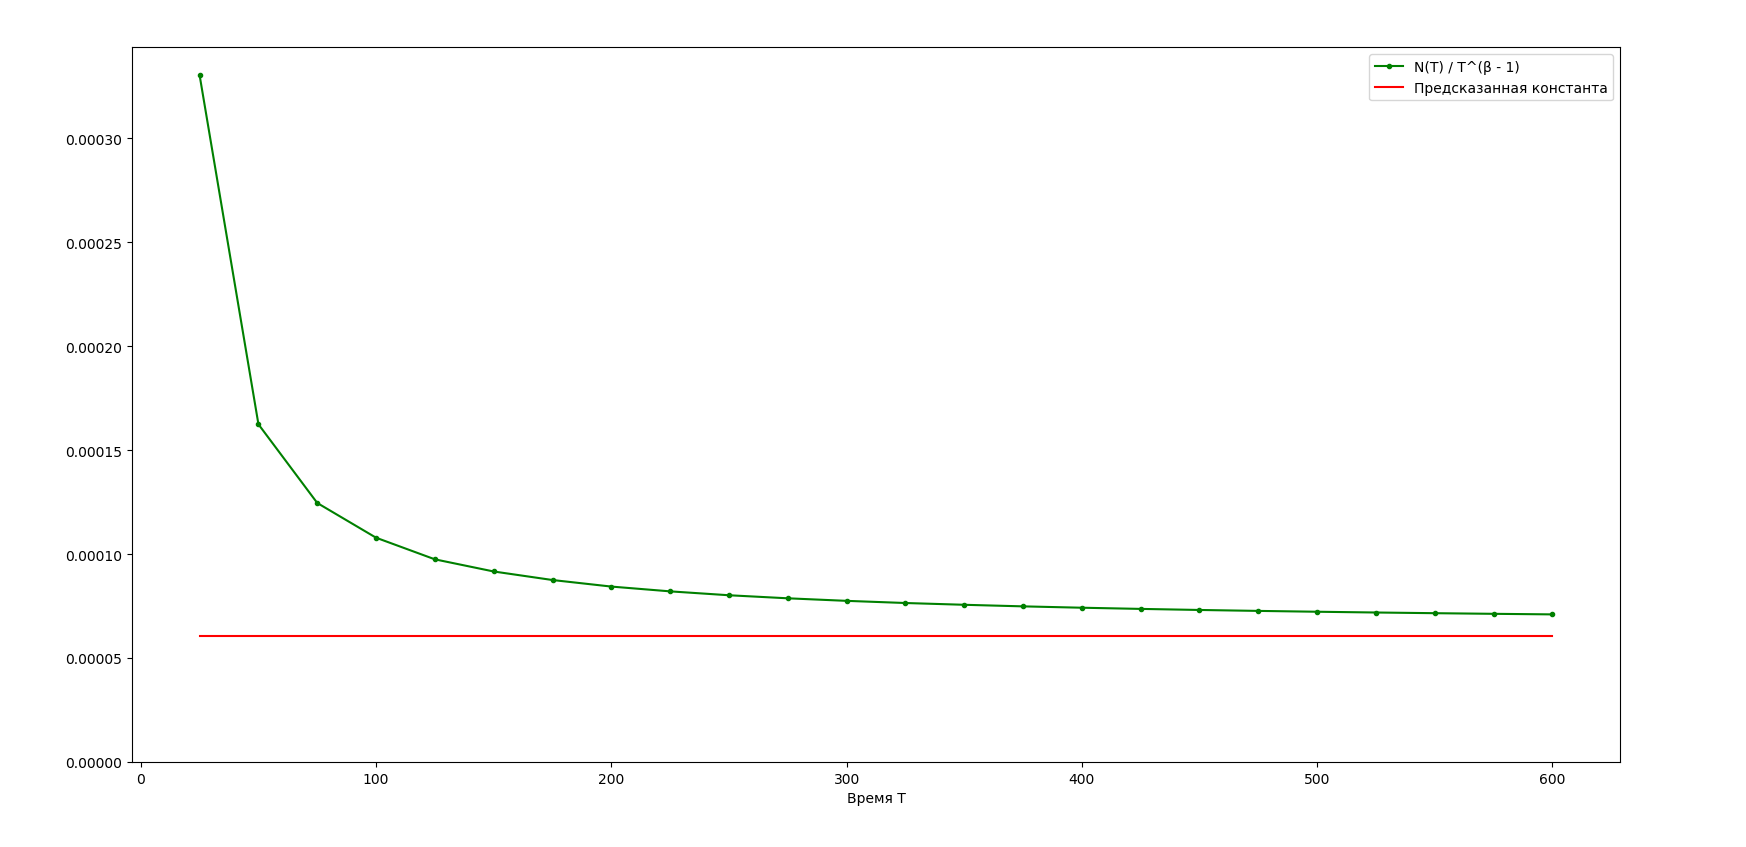
\includegraphics[scale=0.5]{Experiment.png}
\end{center}
\caption{Сходимость $\frac{N(T)}{T^{\beta - 1}}$}
\end{figure}

\FloatBarrier

Действительно, $\frac{N(T)}{T^{\beta - 1}}$ приближается к $\sum_{d \in D_{\beta}}\frac{\sum_{e \in E}{t(e)}}{(\beta - 1)!\prod_{i = 1}^{\beta}{t(d_{i})}}$ по мере роста $T$.

Теперь давайте рассмотрим еще один способ проверить, что коэффициент посчитан правильно.
Допустим, что $N(T) = aT^{\beta - 1} + bT^{\beta - 2} + O(T^{\beta - 3})$, такое допущение обосновано, поскольку для неориентированных графов доказано (в $\cite{second}$, например), что можно получить второй коэффициент разложения $N(T)$.

Введем следующую функцию:

\begin{gather*}
    h_{c}(T) = \frac{\frac{N(2T)}{(2T)^{\beta - 1}} - c}{\frac{N(T)}{T^{\beta - 1}} - c} \\
\end{gather*}

\begin{gather*}
    h_{a}(T) = \frac{\frac{N(2T)}{(2T)^{\beta - 1}} - a}{\frac{N(T)}{T^{\beta - 1}} - a} = \frac{a + \frac{b}{2T} + O\left(\frac{1}{T^{2}}\right) - a}{a + \frac{b}{T} + O\left(\frac{1}{T^{2}}\right) - a} = \frac{\frac{1}{2} + O\left(\frac{1}{T}\right)}{1 + O\left(\frac{1}{T}\right)}
\end{gather*}

$\lim_{T \to \infty}{h_{a}(T)} = \frac{1}{2}$.

Пусть теперь $a' \neq a$.

\begin{gather*}
    h_{a'}(T) = \frac{\frac{N(2T)}{(2T)^{\beta - 1}} - a'}{\frac{N(T)}{T^{\beta - 1}} - a'} = \frac{a + \frac{b}{2T} + O\left(\frac{1}{T^{2}}\right) - a'}{a + \frac{b}{T} + O\left(\frac{1}{T^{2}}\right) - a'} = \frac{a - a' + O\left(\frac{1}{T}\right)}{a - a' + O\left(\frac{1}{T}\right)}
\end{gather*}

$\lim_{T \to \infty}{h_{a'}(T)} = 1$.

Таким образом, чтобы проверить, что какое-то $c$ совпадает с $a$, достаточно найти значение $h_{c}(T)$ при достаточно больших $T$. Если оно близко к $\frac{1}{2}$, то это хороший кандидат для $a$, иначе если значение близко к $1$, то, скорее всего, это не $a$.

Рассмотрим пример. Граф будет тем же, что и в предыдущем подходе. Возьмем $a' = 0.6 \cdot a \approx 0.6 \cdot 0.00006482629 = 0.000038895774$.

\begin{figure}[!htb]
\begin{center}
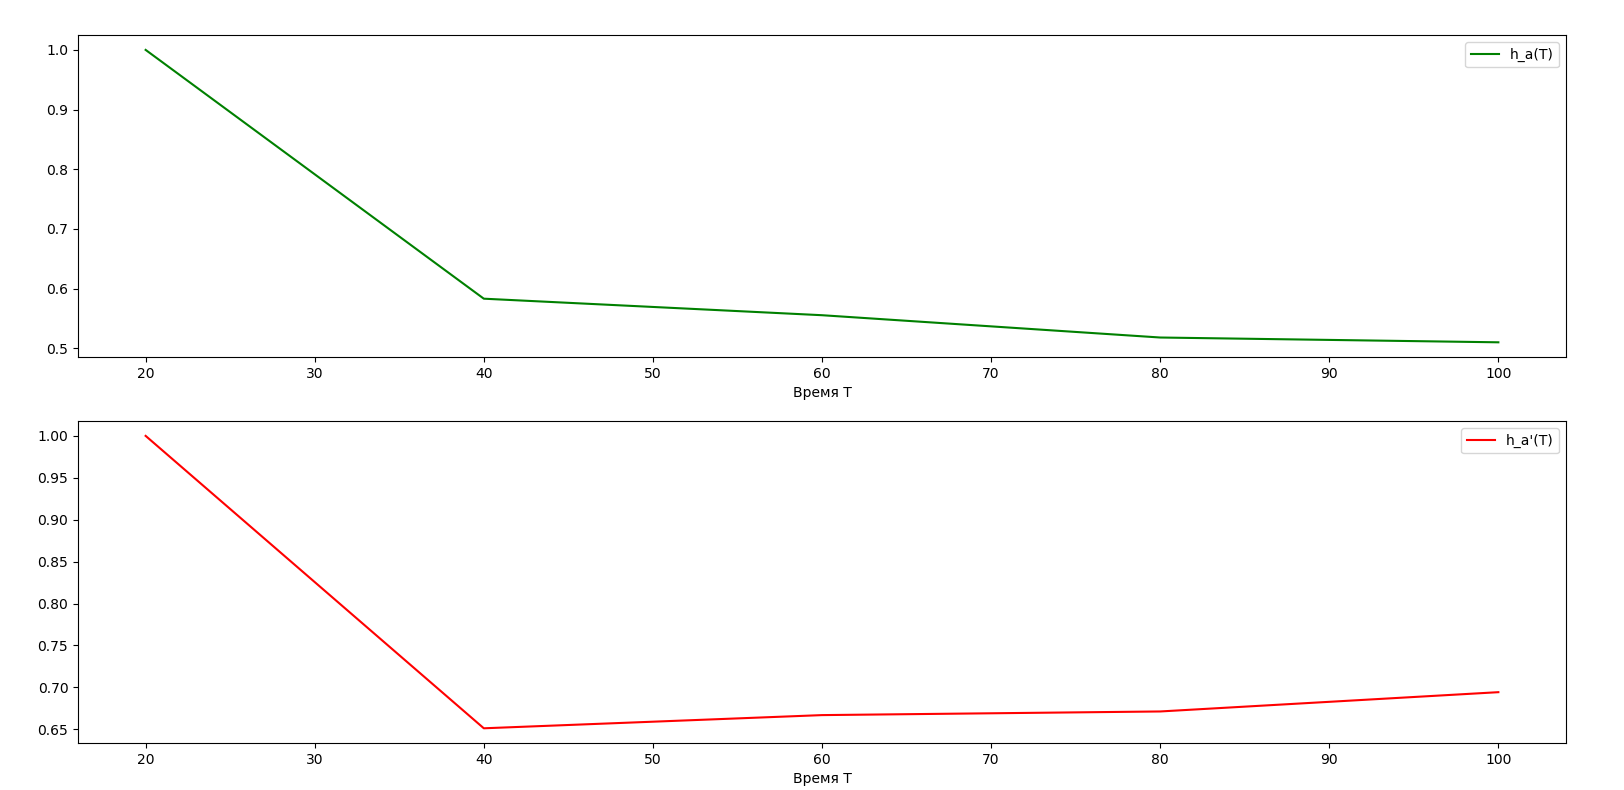
\includegraphics[scale=0.5]{Experiment_2.png}
\end{center}
\end{figure}

\FloatBarrier

Заметим, что $h_{a}(T)$ близка к $\frac{1}{2}$ даже при небольших $T$, в то время как $h_{a'}(T)$ дальше от $\frac{1}{2}$.

\section{Заключение}

Мы нашли асимптотику для $N(T)$ при $T \to +\infty$ для гамильтоновых графов (более точно, графов, которые описаны в секции $1.2$).
Старший коэффициент $\sum_{d \in D_{\beta}}\frac{\sum_{e \in E}{t(e)}}{(\beta - 1)!\prod_{i = 1}^{\beta}{t(d_{i})}}$ не зависит от выбора порядка на ребрах, то есть $\sum_{d \in D_{\beta}}\frac{1}{\prod_{i = 1}^{\beta}{t(d_{i})}}$ является инвариантом относительно смены порядка на ребрах для гамильтоновых графов. Понимание природы этого инварианта и изучение $N(T)$ для ориентированных сильно связных графов, которые не являются гамильтоновыми, могут быть целью для дальнейшего исследования.

\section{Благодарности}
Автор выражает благодарность Всеволоду Леонидовичу Чернышеву за неоценимую помощь в подготовке текста и статьи, идеи которых легли в основу многих подходов из данного текста.
Также автор выражает благодарности Даниилу Эдуардовичу Волгину за предоставление вычислительных ресурсов, которые были использованы для компьютерного моделирования и Дмитрию Александровичу Полякову за конструктивные обсуждения текста.




\bibliographystyle{unsrt}
\bibliography{bibliography}

% Биекция:

% Пусть $t'$ --- время захода в $1$, $c$ --- набор взвешенных достижимых циклов.

% $t' \xleftrightharpoons[\sigma \circ H]{t} c$.

% $\sigma(\omega(t(c))) = c, \squad t(\sigma(K(t'))) = t'$.

% Чтобы посчитать $\#\{t': t' \leq T\}$ достаточно найти $\#\{c: t(c) \leq T\}$. 


\end{document}